\documentclass{beamer}

\title{some title}
\subtitle{subtitle}
\author{Troy Astorino, Neil Forrester}
\date{April 10, 2013}
\institute[6.834 -- MIT]{Cognitive Robotics \\ Massachusetts Institute of Technology}

\usepackage{graphicx}

\usetheme{CambridgeUS}
\usecolortheme{beaver}
\setbeamertemplate{section in toc}[square]
%\setbeamercolor{section number projected}[bg=black, fg=red]
\setbeamertemplate{navigation symbols}{} % remove navigation symbols

% macros for including shape pictures at various scales (Large, Medium, Small)
\def \spL [#1]{\includegraphics[scale=0.5]{img/#1.png}}
\def \spM [#1]{\includegraphics[scale=0.3]{img/#1.png}}
\def \spS [#1]{\includegraphics[scale=0.15]{img/#1.png}}

\begin{document}

\begin{frame}
	\maketitle
\end{frame}

\begin{frame}
	\frametitle{Outline}
	\tableofcontents
\end{frame}

\section{section title}
\begin{frame}
	\frametitle{Why do we need manipulation-based search for occluded
          objects?}
        \begin{figure}
          \centering
          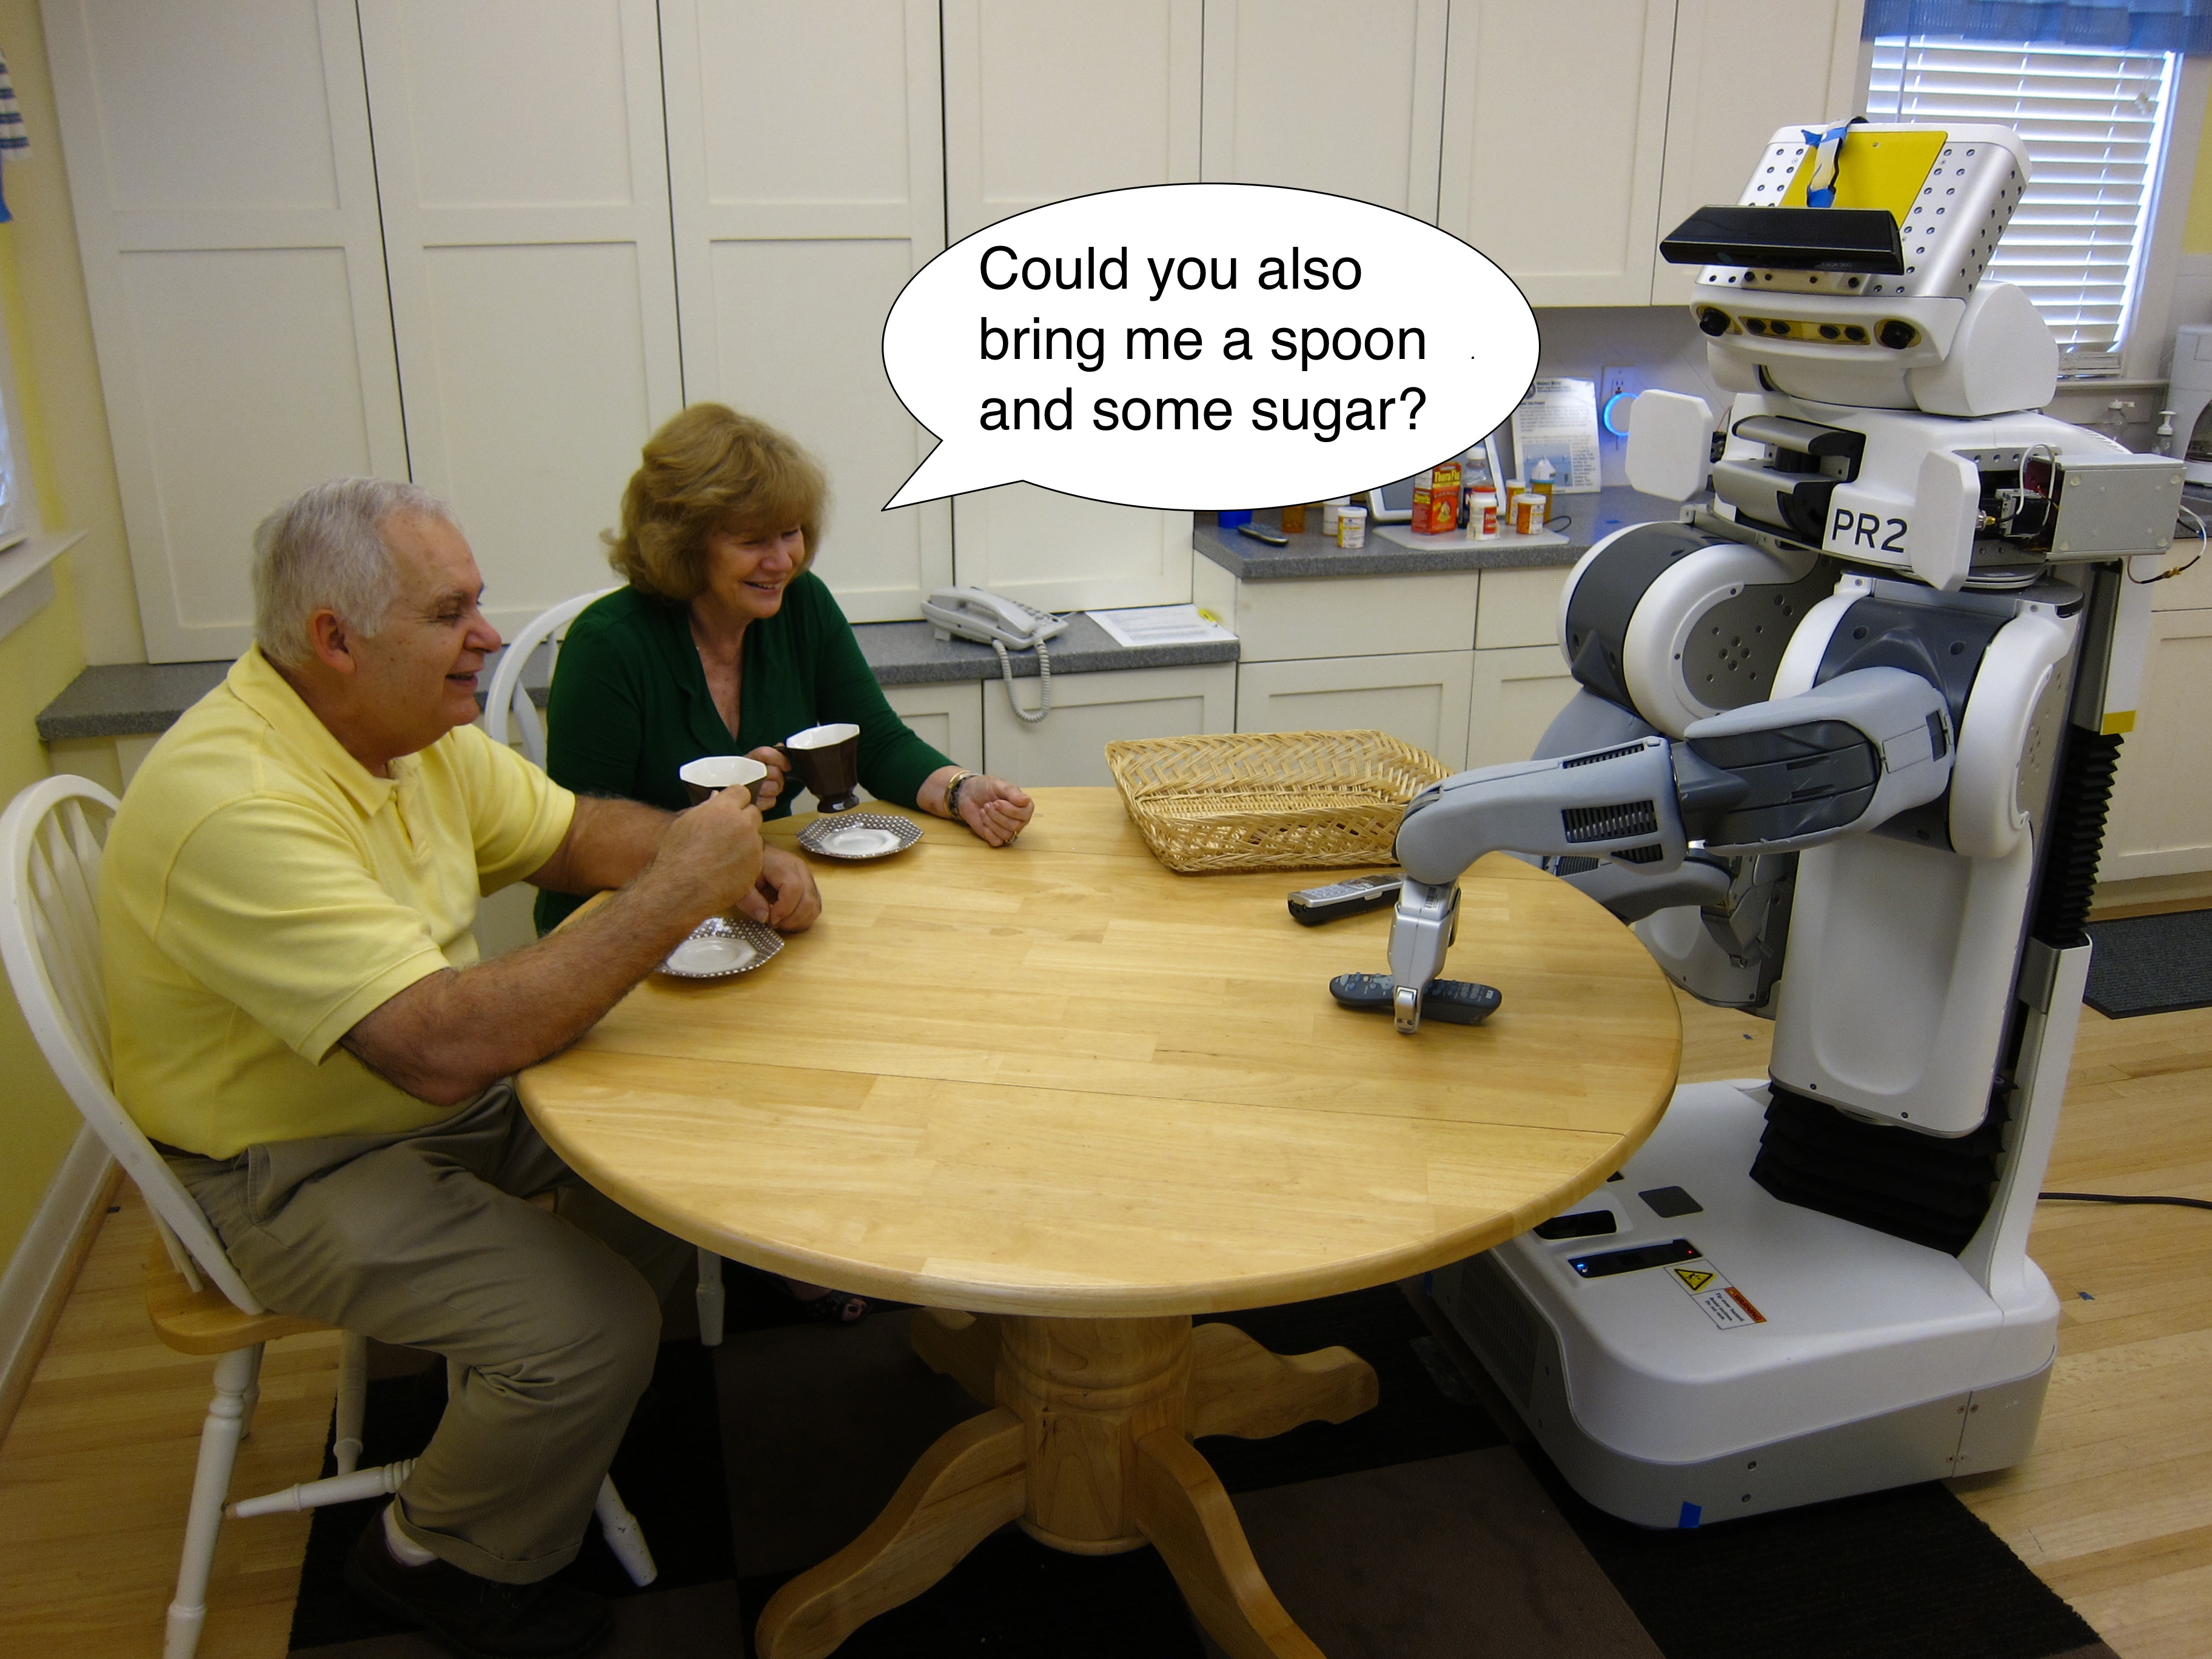
\includegraphics[width=3.2in]{img/robot_in_kitchen.jpg}

          \tiny{Original image courtesy of Wendy Rogers/Georgia Tech}
        \end{figure}
\end{frame}

\section{Generative Model of Container Contents}
\begin{frame}
	\frametitle{The Problem}
	\begin{center}
		\vspace{-0.13in}
		Set of containers: $\{c_l\}$

		\spL[3-unknown-containers]

		Set of object types: $\{t_i\}$

		\spL[shape-universe-small]

		We want to find an object of type $q$ (the query type).

		\spL[blue-circle]

	\end{center}
\end{frame}

\end{document}
